\documentclass[12pt]{article}
\usepackage[margin=1.5cm]{geometry} 
\usepackage{graphicx}
\usepackage{amsmath,amsthm,amssymb}
\usepackage{hyperref}

\title{
    \textbf{CS3563: DBMS II} \\ 
    \textbf{Group 9 Project Report} \\
}

\author{
    \small
    \begin{tabular}{c}
        \textbf{Darpan Gaur} \\
        \textbf{CO21BTECH11004}
    \end{tabular}
    \begin{tabular}{c}
        \textbf{Abhinav Kompella} \\
        \textbf{ES21BTECH11002}
    \end{tabular}
    \begin{tabular}{c}
        \textbf{Aditya Bacharwar} \\
        \textbf{ES21BTECH11003}
    \end{tabular}
    \begin{tabular}{c}
        \textbf{Avaneesh Radhakrishnan} \\
        \textbf{ES21BTECH11022}
    \end{tabular}
}


\date{}

\begin{document}
\maketitle

\hrulefill

\section*{Introduction}
The Job Portal system serves as a platform that bridges job seekers and employers. We have developed a web-based application for job seekers and employers to connect with each other. Job seekers can create profiles, browse job listings, apply for positions, and track the status of their applications. Employers can post job openings, review applications, and manage candidate information efficiently. The system also provides notifications to keep users informed about relevant events.

\section*{Database Design}
ER Diagram: Figure \ref{fig:ER Diagram} shows the ER Diagram of the database.
The following tables are present in the database:
\begin{itemize}
    \item CustomUsers
    \item JobsListing
    \item JobApplications
    \item RecruitingCompany
    \item Applicant
    \item Resume
    \item Notification
    \item JobStatus
    \item Location
    \item Industry
    \item Skills
\begin{figure}[h]
    \centering
    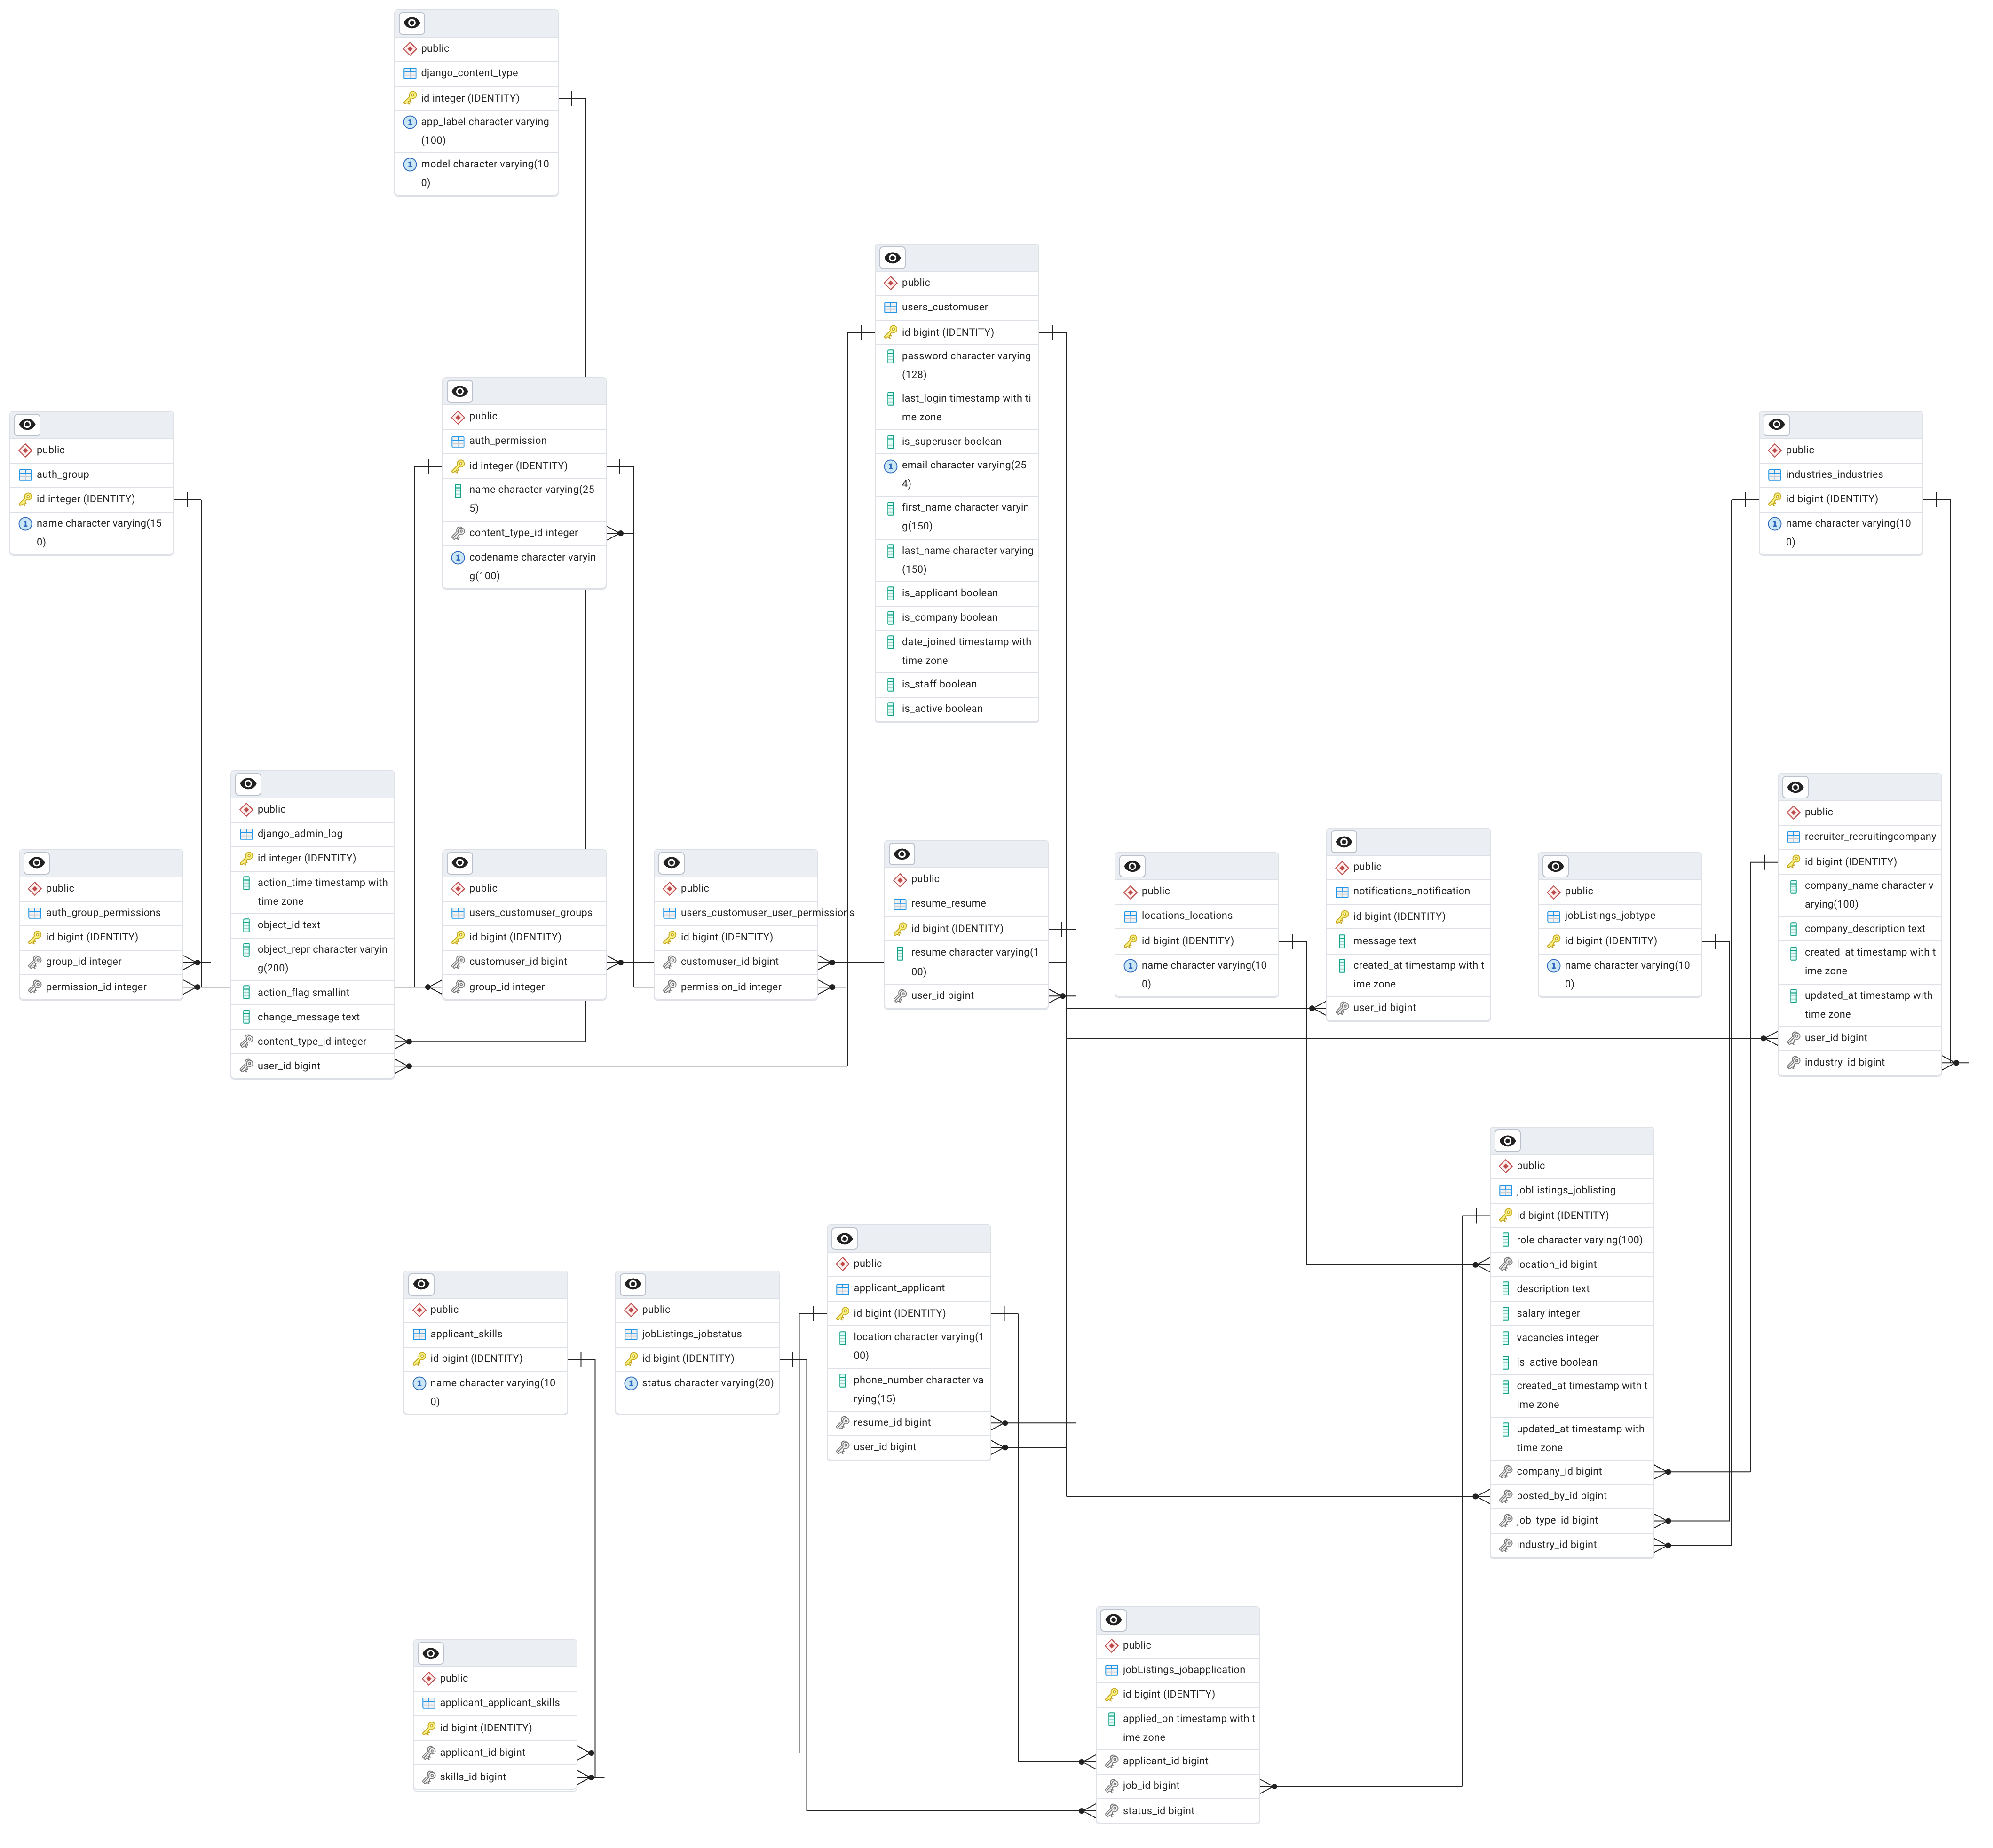
\includegraphics[width=1.0\textwidth]{../images/ERD.png}
    \caption{ER Diagram}
    \label{fig:ER Diagram}
\end{figure}

\subsection*{Functional Dependencies}
\begin{itemize}
    \item User\_id $\implies$ Email, Password, Mobile \quad [\texttt{Users Table}]
    \item Job\_id $\implies$ Role, Description, Salary, Vacancy, Location, Industry, Company\_id [\texttt{JobsListing Table}]
    \item Application\_id $\implies$ User\_id, Resume\_id, Job\_id, Status [\texttt{Applications Table}]
    \item Industry\_id $\implies$ Industry\_name [\texttt{Industry Table}]
    \item Company\_id $\implies$ Company\_name, Company\_description [\texttt{Company Table}]
\end{itemize}

\section*{Technology Stack}
\begin{itemize}
    \item Frontend: HTML, CSS, JavaScript
    \item Backend: Django (Python)
    \item Database: PostgreSQL
\end{itemize}

\section*{Functionality}
\begin{itemize}
    \item User Registration/Sign-up/Login and Authentication
    \begin{itemize}
        \item Implemented CustomUser Model extending AbstractBaseUser provided by Django, to allow users to login using email. Used Highly Secure Django's Authentication System for user authentication.
        \item Extended User Sign-up to For Different Registration of Job Seeker and Job Provider.
        \item This kind of Role-based Authentication allowed us to implement Role Based Access Control.
    \end{itemize}
    \item Job Seeker
    \begin{itemize}
        \item Job Seeker can create a profile with relevent details, upload resume, and apply for jobs.
        \item Job Seeker can search for jobs based on location, Job Title, Company Name, Industry, etc.
        \item Job Seeker can view and manage their job Application at one place. Allowing applicant Withdrew Application, View Application Status and other job relevent job details.
        \item Job Seeker can view the list of jobs they have applied for.
    \end{itemize}
    \item Job Recruiter
    \begin{itemize}
        \item Job Recruiter can create company profile with relevent details, and post jobs.
        \item Job Recruiter can view and manage their job postings at one place. Allowing recruiter to Edit Job Posting, Delete Job Posting, View Job Posting Status and other job relevent job details.
        \item Job Recruiter can view the list of job seekers who have applied for their job postings.
    \end{itemize}
    \item Notifications
    \begin{itemize}
        \item User recieves notifications for various events like job posting, apllication status updates, etc.
        \item Recruiters recieve notifications when a job seeker applies/withdraws from their job posting.
    \end{itemize}
    \item Job Listing
    \begin{itemize}
        \item All the jobs are listed on the home page.
        \item Jobs can be filtered based on location, job title, company name, industry, etc.
        \item Users can see the details of the job and apply for it.
    \end{itemize}
    \item Resume Upload: Can upload resume in pdf format, and use that to apply for jobs directly.
    \item Additional tables: Support for additional tables like Industry, Location, Skill, etc.
\end{itemize}

\section*{Challenges Faced}
\begin{itemize}
    \item Implementing RBAC: To allow different users to access different parts of the application.
    \item Normalizing the database: To reduce redundancy and improve performance.
    \item Debugging: As lot of components were interacting with each other, it was difficult to debug the application.
\end{itemize}

\section*{Future Work}
\begin{itemize}
    \item AI based job recommendation system
    \item Resume Parsing and auto-filling application form
\end{itemize}

\section*{Conclusion}
We have successfully implemented a Job Portal System that allows job seekers and employers to connect with each other. The system provides a user-friendly interface for users to interact with the application.

\end{document}